\section{Functional Structure of Adapter Compression}
\label{sec:diagnostics}
% Section de diagnostics et Interprétation: 
% À nombre de bits comparable, qu’est-ce qui détermine le coût comportemental d’une erreur de compression ?
%how we compress ->
%how we measure preservation->
%why weight error fails->
%why bit location matters

In this section, we examine how adapter compression affects fine-tuned behavior. We use controlled post-training compression to separate numerical reconstruction from functional preservation. Across these diagnostics, intuitive proxies such as weight-space error and nominal bit allocation fail to fully explain the resulting degradation, indicating that compression acts through a structured interaction between the learned update and the frozen model.




\subsection{Experimental Setting: Adapter Compression}

We compress LoRA adapters trained on frozen models from 0.5B to 32B
parameters: Qwen2.5-\{0.5B, 1.5B, 3B, 7B, 14B, 32B\}, Qwen3-8B-Base,
Mistral-7B-v0.1, Llama-3.1-8B and Gemma-2-9B, mostly Qwen2.5-7B. Each
adapter is trained once and compressed at a range of operating points,
without retraining. At one bit per value and above, we
quantize the LoRA factors row-wise; below one bit, we additionally remove
paired rank directions. For every operating point, the compressed
representation and its decoding metadata are serialized to disk, reloaded,
and evaluated as part of the composed model. We report realized file size
normalized by the number of scalar values in the uncompressed adapter,
rather than nominal precision. Full training configurations, codec details,
datasets, and evaluation procedures are given in
Appendix~\ref{app:xp_details}.


\subsection{Measuring Compression Through Behavior}

The object we want to preserve is not the adapter itself, but the behavior
added by fine-tuning. We therefore evaluate compression by how much of the
learned improvement survives after the compressed adapter is reloaded.
Because every operating point comes from the same trained checkpoint, this
isolates the effect of compression from variation in optimization.
\newline
Let $L_0$ denote the held-out loss of the frozen model,
$L_{\mathrm{raw}}$ that of the uncompressed adapter, and $L_r$ the loss after
compression to realized rate $r$. We define retained gain as
\begin{equation}
    \mathrm{Retain}(r)
    =
    \frac{L_0-L_r}{L_0-L_{\mathrm{raw}}}.
    \label{eq:retain}
\end{equation}
Thus, $0$ corresponds to the frozen model and $1$ to the uncompressed adapter;
values above one are possible when compression improves held-out loss.
Normalizing by the raw gain also makes curves comparable across conditions
that learn different absolute amounts.
\newline
Figure~\ref{fig:frontier} shows representative rate-retention curves and the
corresponding threshold summary. For comparisons across conditions, we define
\begin{equation}
    R^\star(\tau)
    =
    \min\{r:\mathrm{Retain}(r)\geq\tau\},
    \label{eq:rstar}
\end{equation}
and use $\tau=0.90$ unless stated otherwise. $R^\star(0.90)$ is therefore an
operational, codec-dependent behavioral rate: the smallest measured reloadable
adapter preserving at least 90\% of the original fine-tuning gain. We defer
the question of what determines shifts in $R^\star$ to
Section~\ref{sec:behavior-prediction}.


\begin{figure}[t]
\centering
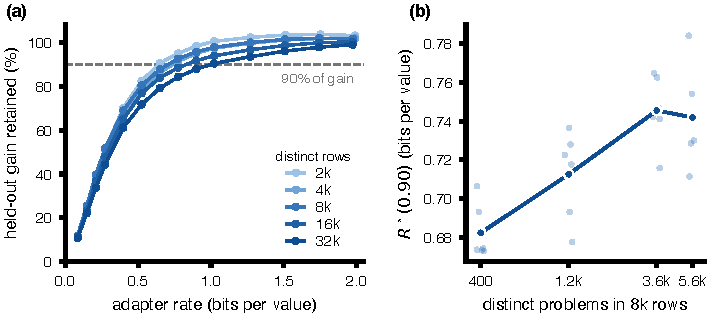
\includegraphics[width=0.75\linewidth]{figures/F2_frontier.pdf}
\caption{
\textbf{Behavioral rate--retention frontier.}
(a) Retained fine-tuning gain versus exact serialized adapter rate across
2k--32k MetaMathQA rows at fixed compute.
(b) $R^\star(0.90)$ at 8k rows as source-problem diversity increases.
Curves show seed means; small points are individual seeds.
Mistral-7B, NF4, rank-16 LoRA.
}
\label{fig:frontier}
\end{figure}

\subsection{Weight Reconstruction Does Not Predict Behavior}

A natural compression objective is to minimize numerical reconstruction error.
If weight-space fidelity were a reliable proxy for functional preservation,
then, at fixed rate, a codec with lower reconstruction error should also
preserve more of the learned behavior.
\newline
We test this by comparing uniform quantization with an adaptive allocator that
selects the precision of each LoRA row to minimize reconstruction error under
a rate constraint, and may remove rows entirely. Additional codec details and
controls are given in Appendix~\ref{app:xp_details}.
\newline
Figure~\ref{fig:weight-error} gives a direct counterexample. Near one bit per
value, the adaptive code achieves lower relative weight RMSE than uniform
quantization (0.54 versus 0.56), yet retains only 3\% of the held-out gain,
compared with 86\% for the uniform code. It obtains the lower error partly by
removing rows that are cheap under the Euclidean objective but behaviorally
important; at higher rates, once rows are no longer removed, the two codecs
converge.
\newline
Thus, lower parameter-space distortion need not imply lower behavioral
distortion. Numerical reconstruction alone does not identify which
perturbations are harmless once the adapter is composed with the frozen model.

\begin{figure}[t]
\centering
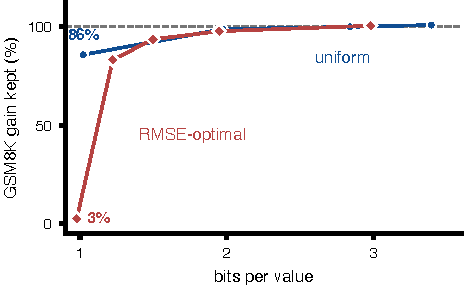
\includegraphics[width=0.47\linewidth]{figures/F3_weight_error.pdf}
\caption{
\textbf{Lower weight error need not preserve more behavior.}
Near one bit per value, the RMSE-optimized codec attains lower relative
weight error than uniform quantization (0.54 vs.\ 0.56) but retains only
3\% of the GSM8K gain, versus 86\% for uniform quantization.
Mistral-7B, NF4, rank-16 LoRA, three seeds.
}
\label{fig:weight-error}
\end{figure}


The location of an error matters as well as its size: at matched budgets,
removing precision from the last third of the layers costs more of the gain
than removing it uniformly, although the update's magnitude is flat across
depth (Appendix~\ref{app:layer-location}). Neither total parameter error nor
total bit budget sets the behavioral cost of compression. If compression acts
unequally on the components of an update, it may also remove harmful
structure while keeping useful behavior; Section~\ref{sec:recovery} shows
that it does.
